\subsection{Autoencoders} \label{sec:Autoencoders}
Over the last decade, autoencoders have been thought of as potentially useful for compression and decompression. 
In practice, though, autoencoders are not ideal for compressing e.g. images or sound - and have failed to replace compression algorithms such as \texttt{JPEG} and \texttt{MP3}.
Autoencoding procedures are best suited for tasks that require data-specificity - i.e. an autoencoder trained to compress images of cats, typically will not do well in compressing images of cars. 
\newline
Autoencoders are commonly used for data-denoising, e.g. removing static noise from images. 
Autoencoders are also utilized for their ability to compress information into a smaller space - this can be useful in generating visualizations and computing similarity of high-dimensional data. 
\newline
Autoencoders come in many different varieties; sparse, stacked, denoising, deep, convolutional, variational, etc. Each of these have their own drawbacks and merits and some of these will be discussed further.

Within the field of machine learning, an autoencoder refers to a neural network architecture which is trained to replicate its input to its output\autocite{Bengio2009}.

An autoencoder utilizes an encoder, which compresses its input to a lower dimension vector - and a decoder that seeks to replicate the original input from this lower dimension representation.
Autoencoders are symmetrical in that the encoding layer is mimicked in the decoding layer as an inverted version of the encoding layer.

\begin{figure}[H]
    \centering
    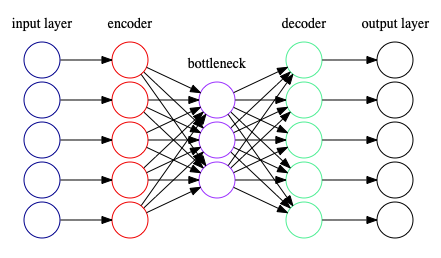
\includegraphics[scale=0.4]{pictures/graphviz/autoencoder_simple}
    \caption{Quintessential autoencoder architecture}
    \label{fig:simpleautoencoder}
\end{figure}

Formally, this can represented as follows: The autoencoder takes an input and maps that into a hidden representation (bottleneck) using an encoder. This happens via a deterministic mapping: 
$$
x\in[0,1]^{d} \xrightarrow{\text{$f(x)$}} y\in[0,1]^{d'}, \quad \quad f(x) = s(Wx + b)
$$
where $s$ represents a non-linear activation function; e.g. \texttt{sigmoid} or \texttt{ReLU}. 
From this, the decoder maps $y$ into $z$, where $z$ is an attempt at reconstructing $x$ from $y$; $x$ and $z$ are of same shape. This occurs through a mapping that is inverted from the mapping stated above:
$$
y\in[0,1]^{d'} \xrightarrow{\text{$f'(y)$}} z\in[0,1]^{d}, \quad \quad f'(x) = s(W'y + b')
$$
The weights, $W, W'$ are tuned to minimize the error rate of the reconstruction $z$ compared to the original input, $x$. A commonly used reconstruction error is the Mean Squared Error(\texttt{MSE}).
We denote the MSE as:
$$
L(xz) = ||x-z||^{2}
$$

Penalizing the autoencoder towards minimizing the reconstruction error is an effort towards achieving a hidden representation, $y$, that captures the most important features of the data.
As such, the autoencoder is trained to distill the input data in a way, that it can still be reconstructed from $y$ with the least amount of data fidelity loss in $z$.

The autoencoders hidden representation does not retain perfect information - and is as such a lossy compression of $x$. 
The encoder is optimized towards compressing the data on which it is trained, and as such, autoencoders do not generalize well. 

\subsection{Denoising Autoencoders}
A denoising autoencoder is similar to any autoencoder in form, with the distinction, that the input to a denoising autoencoder is corrupted prior to training.
Also, the reconstruction error is computed by comparing the reconstruction, $\widetilde{z}$ to the non-corrupted input, $x$. 
Thus, the autoencoder is trained to denoise the corrupted input, $\widetilde{x}$. In line with notation from \autoref{sec:Autoencoders}, we can describe the denoising autoencoder as:

$$
\widetilde{x} \sim q_{D}(\widetilde{x}|x) 
$$
$$
\widetilde{x}\in[0,1]^{d} \xrightarrow{\text{$f(\widetilde{x})$}} \widetilde{y}\in[0,1]^{d'}, \quad \quad f(\widetilde{x}) = s(W\widetilde{x} + b)
$$
$$
\widetilde{y}\in[0,1]^{d'} \xrightarrow{\text{$f'(\widetilde{y})$}} \widetilde{z}\in[0,1]^{d}, \quad \quad f'(\widetilde{y}) = s(W'\widetilde{y} + b')
$$

The \texttt{MSE} can then be computed as:
$$
L(x\widetilde{z}) = ||x-\widetilde{z}||^{2}
$$

One way of defining the corruption, $q_{D}$, is zeroing out random values\autocite{Vincent2008}, commonly referred to as salt-and-pepper noise in greyscale images.

A denoising autoencoder is due to its ability to reconstruct tainted input a more robust version of the autoencoder, and is thought to be slightly more generalizable than the standard autoencoder, \autoref{sec:Autoencoders}.

\subsection{Deeper Autoencoders}
An autoencoder model is said to be deep when the encoder and decoder parts, respectively, are constructed of multiple layers - often fully-connected or convolutional layers. 
Deep autoencoder architectures have shown to be proficient at mapping images to meaningful hidden representations\autocite{Krizhevsky2010}. 

\begin{figure}[H]
    \centering
    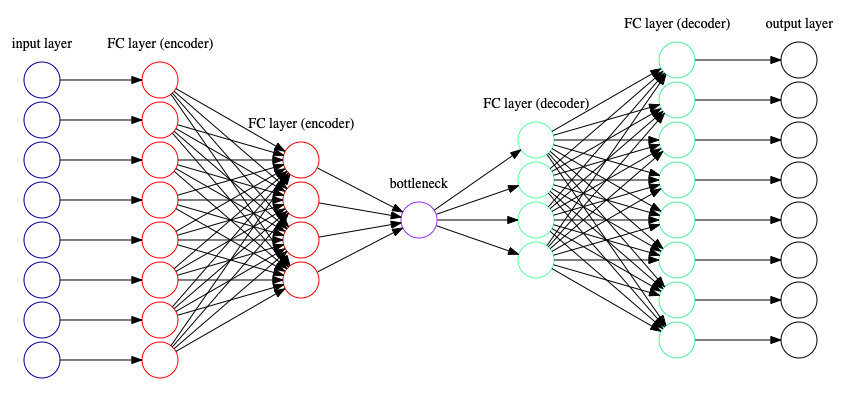
\includegraphics[scale=0.4]{pictures/graphviz/autoencoder_deep}
    \caption{Example of Deep Autoencoder architecture}
    \label{fig:deepautoencoder}
\end{figure}

Deeper autoencoders may have the capacity to capture more intricate mechanisms, allowing for better performance in some tasks at the cost of higher training cost and risk of overfitting. 
In older literature, it is suggested to do greedy layer-wise training of deeper autoencoder architectures - as we will see in \autoref{sec:trainae} better approaches have since been established.
\newline



